% Compile:
%   pdflatex hedonic_baseline_report.tex
% or:
%   latexmk -pdf hedonic_baseline_report.tex
%
% Notes:
% - This document focuses on the hedonic regression baseline (Model 1).
% - For an overall comparison across all models, see `REPORT.md` and `report.tex`.
% - For interactive plots with one-click PNG/SVG downloads, open `plots/report_graphs.html`.

\documentclass[11pt]{article}

\usepackage[margin=1in]{geometry}
\usepackage{microtype}
\usepackage{amsmath}
\usepackage{booktabs}
\usepackage{graphicx}
\usepackage{siunitx}
\usepackage{enumitem}
\usepackage{xcolor}
\usepackage{hyperref}
\usepackage{pgfplots}
\usepackage{pgfplotstable}
\usepackage{subcaption}
\usepackage{longtable}
\usepackage{tabularx}
\usepackage{array}
\usepackage{listings}

\pgfplotsset{compat=1.18}
\sisetup{detect-weight=true, detect-family=true}
\hypersetup{
  colorlinks=true,
  linkcolor=blue!60!black,
  urlcolor=blue!60!black,
  citecolor=blue!60!black
}

\lstset{
  basicstyle=\ttfamily\small,
  breaklines=true,
  columns=fullflexible,
  frame=single,
  framerule=0.3pt,
  rulecolor=\color{black!20},
  upquote=true
}

\usetikzlibrary{positioning,arrows.meta,shapes.geometric}

% -----------------------------
% Key numbers (copied from this repo's tensors/results as of 2026-03-12)
% -----------------------------
\newcommand{\NTotal}{597{,}928}
\newcommand{\NTrain}{418{,}549}
\newcommand{\NVal}{89{,}689}
\newcommand{\NTest}{89{,}690}

% Robustness: eval_suite (full features)
\newcommand{\AnnRandRmseMean}{0.1420}
\newcommand{\AnnRandRmseStd}{0.0036}
\newcommand{\AnnRandAccMean}{92.64}
\newcommand{\AnnRandAccStd}{0.31}

\newcommand{\HedRandRmseMean}{0.2446}
\newcommand{\HedRandRmseStd}{0.0030}
\newcommand{\HedRandAccMean}{87.76}
\newcommand{\HedRandAccStd}{0.10}

\newcommand{\AnnTimeRmseMean}{0.3146}
\newcommand{\AnnTimeRmseStd}{0.0365}
\newcommand{\AnnTimeAccMean}{82.78}
\newcommand{\AnnTimeAccStd}{2.35}

\newcommand{\HedTimeRmseMean}{0.5947}
\newcommand{\HedTimeRmseStd}{0.0162}
\newcommand{\HedTimeAccMean}{69.35}
\newcommand{\HedTimeAccStd}{1.09}

% Representative best single hedonic run (full features, full train).
\newcommand{\HedBestTestRmse}{0.2428}
\newcommand{\HedBestTestAcc}{87.74}

% -----------------------------
% Inline data tables used by pgfplots (representative hedonic run, seed=42)
% These were generated by training `hedonic_baseline.py` for 20 epochs on the
% full feature set with a 70/15/15 random split (seed=42).
% -----------------------------

\pgfplotstableread[col sep=space]{
epoch trainrmse valrmse valacc
1 10.753809 7.729551 0.044554
2 5.718912 3.650199 2.672553
3 2.515295 1.418394 25.853533
4 0.939612 0.542972 67.064932
5 0.420779 0.360375 82.740185
6 0.335837 0.333668 83.570135
7 0.317222 0.320016 84.134097
8 0.303782 0.308141 84.743692
9 0.292135 0.298257 85.309449
10 0.281952 0.290065 85.773595
11 0.273344 0.282567 86.101179
12 0.266010 0.276476 86.434530
13 0.259734 0.271280 86.707059
14 0.254225 0.266904 86.976969
15 0.249684 0.263444 87.217480
16 0.245268 0.259524 87.211530
17 0.241709 0.256973 87.359129
18 0.238433 0.254131 87.522760
19 0.235496 0.251843 87.624721
20 0.232944 0.250032 87.792444
}\HedCurve

\pgfplotstableread[col sep=space]{
center count
-0.975 86
-0.925 104
-0.875 108
-0.825 114
-0.775 152
-0.725 178
-0.675 243
-0.625 303
-0.575 412
-0.525 509
-0.475 666
-0.425 900
-0.375 1283
-0.325 1783
-0.275 2514
-0.225 3455
-0.175 4892
-0.125 6551
-0.075 8143
-0.025 9466
0.025 10174
0.075 9911
0.125 8555
0.175 6391
0.225 4441
0.275 2771
0.325 1695
0.375 1103
0.425 680
0.475 448
0.525 302
0.575 221
0.625 164
0.675 100
0.725 99
0.775 72
0.825 43
0.875 48
0.925 30
0.975 15
}\HedResidHist

\pgfplotstableread[col sep=space]{
true pred
13.474429 13.551935
12.861001 12.836718
15.228447 15.166054
13.746161 13.615883
12.694655 12.629995
13.426167 13.367037
12.945628 12.903193
12.535380 12.816313
14.187075 14.388914
12.989977 12.817617
13.656516 13.593847
14.607598 14.406498
13.244583 12.938261
13.190023 13.113356
13.099710 13.264223
12.506181 12.783075
13.178745 13.006716
13.343907 13.109009
12.358798 12.933941
12.771389 12.594215
13.180634 13.213421
13.415034 13.165525
13.712925 13.435469
13.668751 13.446287
12.691584 12.830135
13.444448 13.239460
14.220976 14.189880
12.528160 12.514797
13.475835 13.251270
12.644331 11.983820
13.361382 13.423531
14.138319 14.108438
13.127353 13.179224
13.514407 13.575445
13.361382 13.423723
12.884109 13.128784
13.407544 13.152824
13.737550 13.710833
12.861001 13.092505
13.296318 13.295591
12.951577 13.000008
13.586099 13.482718
13.060490 13.155104
13.635188 13.294823
13.171155 13.205034
13.537780 13.538286
14.316286 14.182791
13.235694 13.229116
13.681980 14.152966
13.269059 13.042036
13.820499 13.837618
14.731802 13.543854
13.180634 13.129059
13.380876 12.808104
14.038655 13.812187
13.366096 12.781050
12.827995 12.886337
12.943000 13.158807
12.560248 11.839235
12.785213 12.672733
12.366920 12.459249
11.938200 12.200367
13.549630 13.604620
13.981026 14.201624
13.487008 13.358616
13.051407 12.890869
13.132316 13.242641
12.971542 13.399012
14.039454 14.258608
13.384729 13.716196
13.089636 13.072624
13.260386 13.016668
12.611541 13.361027
12.923915 12.719194
13.302685 13.295712
13.338283 13.059437
14.054528 14.160391
12.362226 12.250008
13.393155 13.479033
13.055157 12.901184
13.337477 12.975397
13.038984 13.193144
13.369225 13.215460
12.230770 12.590265
13.556741 13.658970
13.132316 12.868738
13.315626 13.099295
13.441545 13.397438
12.542548 12.417885
12.570719 12.784184
13.849913 13.930681
12.470362 12.345167
13.536987 13.049831
14.014362 13.482027
12.796636 12.662210
14.040653 13.885809
13.381647 13.651966
13.610945 13.451525
13.353477 13.085676
13.422469 13.384876
12.542548 12.793383
14.445719 14.217363
13.715692 13.536531
13.623140 13.316212
12.911398 13.028694
12.577640 12.853266
12.988834 12.959496
11.571204 12.209780
12.873648 13.114594
13.081544 12.958242
14.046623 13.387707
12.873648 12.917772
13.233907 13.088314
12.765692 12.929537
13.279368 13.173149
12.663184 12.761213
13.784021 13.376703
14.004891 13.458323
13.226726 13.303810
13.785052 13.739502
15.173663 15.361700
12.165256 12.272861
12.575914 15.006784
13.287880 13.338659
13.132316 13.194170
14.172486 14.000090
13.369069 13.316193
13.056226 13.228203
13.019225 13.025219
13.353477 13.590645
12.736704 12.554337
12.487489 12.265762
13.220399 13.193567
14.220976 13.741732
12.736704 12.671892
13.204866 13.224058
13.480040 13.418274
12.522710 12.069386
13.106236 13.114834
13.199327 13.280638
14.346727 14.271429
13.102162 13.125542
13.384729 13.435671
14.408838 14.236778
13.167338 13.061001
13.963931 13.999918
12.699246 12.713276
13.038984 13.111769
13.049795 12.953785
13.215856 13.297749
}\HedScatter

\pgfplotstableread[col sep=space]{
year acc mdape n
2010 86.777057 13.222943 7414
2011 86.897796 13.102204 8798
2012 87.828939 12.171061 8855
2013 87.355794 12.644206 8339
2014 87.068191 12.931809 9755
2015 88.201318 11.798682 10545
2016 88.583807 11.416193 11446
2017 86.874361 13.125639 10194
2018 89.457521 10.542479 7279
2019 89.049383 10.950617 4251
}\HedByYear

\pgfplotstableread[col sep=space]{
decile acc mdape n lo hi
1 86.471273 13.528727 8959 308.0 816.0
2 86.155239 13.844761 8316 816.0 1050.0
3 87.281013 12.718987 8543 1050.0 1200.0
4 87.881379 12.118621 9430 1200.0 1350.0
5 88.833055 11.166945 9314 1350.0 1550.0
6 89.626279 10.373721 6859 1550.0 1714.3
7 88.083012 11.916988 11242 1714.3 1950.0
8 88.931307 11.068693 8891 1950.0 2300.0
9 87.952232 12.047768 9161 2300.0 2836.0
10 85.147294 14.852706 8975 2836.0 14850.0
}\HedByAreaDecile

\pgfplotstableread[col sep=space]{
fsa eff
M5R 0.638061
M4N 0.621973
M4V 0.587017
M5P 0.561683
M4W 0.560318
M4T 0.535383
M5N 0.515133
M5M 0.502635
K0K -1.055349
L1B -1.055349
L9Y -1.055349
L4N -0.754858
K9A -0.709540
N0H -0.694244
L0K -0.668937
L0M -0.656835
}\HedFsaEffects

\pgfplotstableread[col sep=space]{
splitseed seed rmse acc
7 0 0.249675 87.830174
7 1 0.248027 87.875400
7 2 0.249352 87.777308
7 3 0.247490 87.804008
7 4 0.249071 87.735488
13 2 0.245189 87.770309
13 3 0.243128 87.815421
13 4 0.244738 87.742881
42 0 0.242633 87.719931
42 1 0.240197 87.947007
42 2 0.242437 87.721571
42 3 0.240751 87.765872
42 4 0.242153 87.738983
123 0 0.247562 87.466604
123 1 0.243877 87.662409
123 2 0.245949 87.741822
123 3 0.244137 87.854987
123 4 0.245933 87.630074
2024 2 0.241890 87.837758
2024 3 0.240467 87.690496
2024 4 0.241649 87.811277
}\HedRobustRandom

\pgfplotstableread[col sep=space]{
splitseed seed rmse acc
7 0 0.616849 67.928213
7 1 0.575182 70.415738
7 42 0.583321 70.306250
42 0 0.610566 68.201694
42 1 0.580844 70.230487
42 2 0.605935 68.726799
42 3 0.586421 69.732425
42 4 0.611438 68.113685
42 42 0.581459 70.510837
}\HedRobustTime

\title{Baseline Model: Hedonic Regression (Linear Fixed Effects)\\
\large Model Description, Evaluation, and Comparison to Neural Networks}
\author{RPSAps360 Project}
\date{March 12, 2026}

\begin{document}
\maketitle

\begin{abstract}
This document describes the \textbf{hedonic regression baseline} used in this project for predicting \texttt{TransactionPrice} (trained on \texttt{log1p(price)}), explains why it is a reasonable baseline for housing valuation, and presents quantitative and qualitative results. The baseline is compared to the primary neural model (ANN with categorical embeddings) using both random splits and a time-based split (train earlier years, test later years). All headline results are tracked in a single canonical spreadsheet (\texttt{results\_all.csv}).
\end{abstract}

\tableofcontents
\newpage

\section{Baseline model choice (why hedonic regression?)}
\paragraph{Reasonable baseline.}
Hedonic regression is a classic approach in real estate modeling: it decomposes price into additive contributions from property attributes and ``fixed effects'' for categorical factors (e.g.\ neighborhood/location proxies). This makes it a strong baseline that is \emph{not random}, is easy to implement, and is widely used in appraisal/valuation settings.

\paragraph{Minimal tuning.}
The baseline has only a few hyperparameters (epochs, batch size, optimizer learning rate) and trains quickly because it is linear in the standardized numeric features plus per-category offsets.

\section{Model definition (with diagram)}
\subsection{Mathematical form}
We predict in log space:
\[
  \hat{y} = b + w^\top x_{\text{num}} + \sum_{j=1}^{d_{\text{cat}}} \beta^{(j)}[x_{\text{cat},j}],
\]
where \(x_{\text{num}}\) is the standardized numeric feature vector and each categorical column \(j\) contributes a learned fixed effect \(\beta^{(j)}[\cdot]\). At evaluation time we convert back to price via:
\[
  \widehat{\text{price}} = \max(0, \exp(\hat{y}) - 1).
\]

\subsection{Implementation diagram}
\begin{figure}[h]
\centering
\begin{tikzpicture}[
  node distance=10mm,
  box/.style={draw, rounded corners, align=center, inner sep=6pt},
  arrow/.style={-Latex, thick}
]
\node[box] (inp) {Inputs from tensor file\\
\texttt{X\_num} (standardized)\\
\texttt{X\_cat} (category indices)};
\node[box, right=of inp] (num) {Numeric linear layer\\
\(w^\top x_{\text{num}} + b\)};
\node[box, below=of num] (cat) {Categorical fixed effects\\
\(\sum_j \\beta^{(j)}[x_{\text{cat},j}]\)};
\node[box, right=of num, yshift=-9mm] (out) {Output\\
\(\hat{y}=\texttt{log1p(price)}\)};
\node[box, right=of out] (metrics) {Metrics\\
RMSE(log)\\
MdAPE (price)\\
Accuracy\%};
\draw[arrow] (inp) -- (num);
\draw[arrow] (inp.east) -- ++(10mm,0) |- (cat.west);
\draw[arrow] (num.east) -- (out.west);
\draw[arrow] (cat.east) -- ++(12mm,0) |- (out.west);
\draw[arrow] (out) -- (metrics);
\end{tikzpicture}
\caption{Hedonic regression baseline architecture (linear + fixed effects). In code this is \texttt{hedonic\_baseline.HedonicLinear}.}
\label{fig:hedonic-diagram}
\end{figure}

\section{Data and preprocessing (reproducible)}
\paragraph{Data source.}
The dataset originates from the RPS proposal pipeline: appraisal-form XML extracts plus transaction feeds (address/date/price) reconciled into a cleaned CSV (\texttt{cleaned\_transaction\_gtha-2.csv}, kept local).

\paragraph{Tensorization (exact script).}
All experiments use \texttt{prepare\_ann\_tensors.py} to convert the cleaned CSV into a tensor file. For the strongest results we use \texttt{feature\_set=full} (location + time + property attributes). This produces:
\begin{itemize}[leftmargin=*]
  \item \texttt{X\_num} (\texttt{float32}) standardized numeric features,
  \item \texttt{X\_cat} (\texttt{int64}) categorical indices for fixed effects / embeddings,
  \item \texttt{y\_log1p} target (\(\log(1+\text{price})\)),
  \item metadata: numeric mean/std and categorical vocabularies.
\end{itemize}

\paragraph{Dataset size and split.}
The full-feature tensor file contains \textbf{\NTotal} transactions. The default split (70/15/15) yields \textbf{\NTrain} train, \textbf{\NVal} validation, and \textbf{\NTest} test samples.

\section{Experimental setup (comparison to ANN)}
\subsection{Splits}
\begin{itemize}[leftmargin=*]
  \item \textbf{Random split:} standard random 70/15/15 partition.
  \item \textbf{Time split:} sort by (\texttt{TransactionYear}, \texttt{Quarter}) and split by time order to evaluate future generalization.
\end{itemize}

\subsection{Metrics}
We report:
\begin{itemize}[leftmargin=*]
  \item \textbf{RMSE(log):} RMSE in log1p space (lower is better).
  \item \textbf{MdAPE:} median absolute percentage error in price space.
  \item \textbf{Accuracy\%:} \(\max(0,100\cdot(1-\text{MdAPE}))\).
\end{itemize}

\section{Quantitative results}
\subsection{Best baseline performance (full features)}
For the best full-train hedonic baseline run recorded so far:
\begin{itemize}[leftmargin=*]
  \item Test RMSE(log): \textbf{\HedBestTestRmse}
  \item Test accuracy (\%): \textbf{\HedBestTestAcc\%}
\end{itemize}

\subsection{Baseline vs neural model (robustness mean $\pm$ std)}
\begin{figure}[h]
\centering
\begin{subfigure}{0.49\linewidth}
\centering
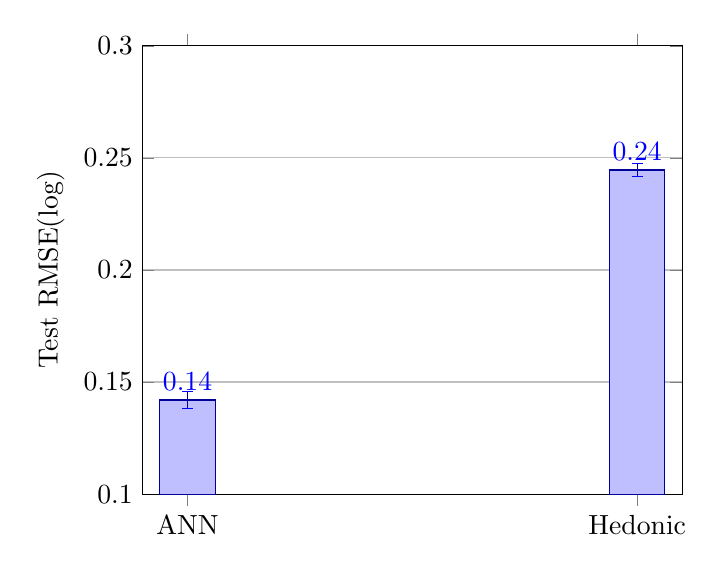
\begin{tikzpicture}
\begin{axis}[
  ybar,
  bar width=20pt,
  ylabel={Test RMSE(log)},
  symbolic x coords={ANN,Hedonic},
  xtick=data,
  ymin=0.10, ymax=0.30,
  ymajorgrids=true,
  error bars/y dir=both,
  error bars/y explicit,
  nodes near coords,
  nodes near coords align={vertical},
]
\addplot+[fill=blue!25, draw=blue!60!black] coordinates {
  (ANN,\AnnRandRmseMean) +- (0,\AnnRandRmseStd)
  (Hedonic,\HedRandRmseMean) +- (0,\HedRandRmseStd)
};
\end{axis}
\end{tikzpicture}
\caption{Random split RMSE(log).}
\end{subfigure}
\hfill
\begin{subfigure}{0.49\linewidth}
\centering
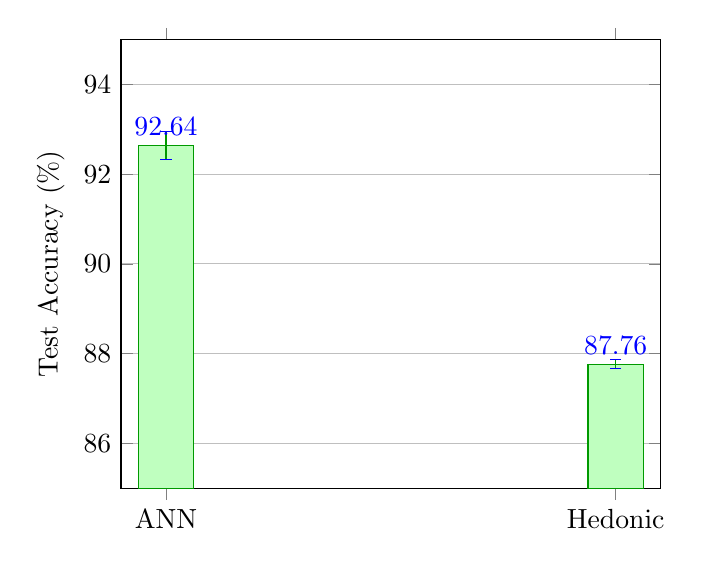
\begin{tikzpicture}
\begin{axis}[
  ybar,
  bar width=20pt,
  ylabel={Test Accuracy (\%)},
  symbolic x coords={ANN,Hedonic},
  xtick=data,
  ymin=85, ymax=95,
  ymajorgrids=true,
  error bars/y dir=both,
  error bars/y explicit,
  nodes near coords,
  nodes near coords align={vertical},
]
\addplot+[fill=green!25, draw=green!60!black] coordinates {
  (ANN,\AnnRandAccMean) +- (0,\AnnRandAccStd)
  (Hedonic,\HedRandAccMean) +- (0,\HedRandAccStd)
};
\end{axis}
\end{tikzpicture}
\caption{Random split accuracy.}
\end{subfigure}

\vspace{2mm}
\begin{subfigure}{0.49\linewidth}
\centering
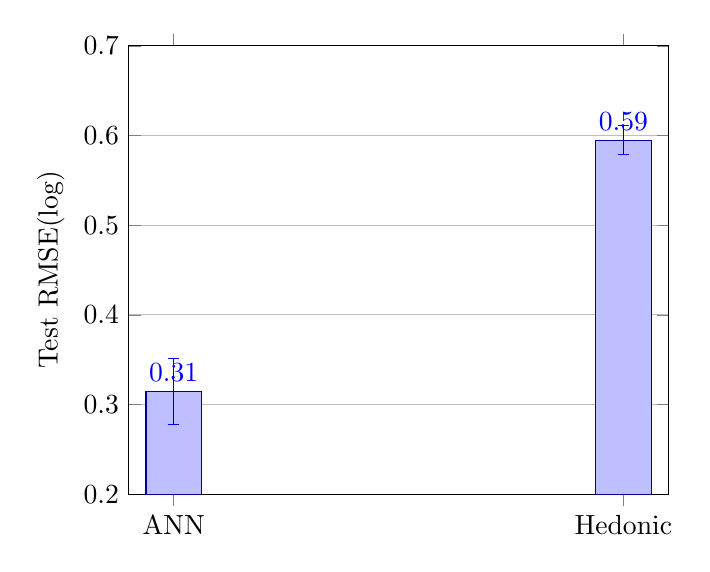
\begin{tikzpicture}
\begin{axis}[
  ybar,
  bar width=20pt,
  ylabel={Test RMSE(log)},
  symbolic x coords={ANN,Hedonic},
  xtick=data,
  ymin=0.20, ymax=0.70,
  ymajorgrids=true,
  error bars/y dir=both,
  error bars/y explicit,
  nodes near coords,
  nodes near coords align={vertical},
]
\addplot+[fill=blue!25, draw=blue!60!black] coordinates {
  (ANN,\AnnTimeRmseMean) +- (0,\AnnTimeRmseStd)
  (Hedonic,\HedTimeRmseMean) +- (0,\HedTimeRmseStd)
};
\end{axis}
\end{tikzpicture}
\caption{Time split RMSE(log).}
\end{subfigure}
\hfill
\begin{subfigure}{0.49\linewidth}
\centering
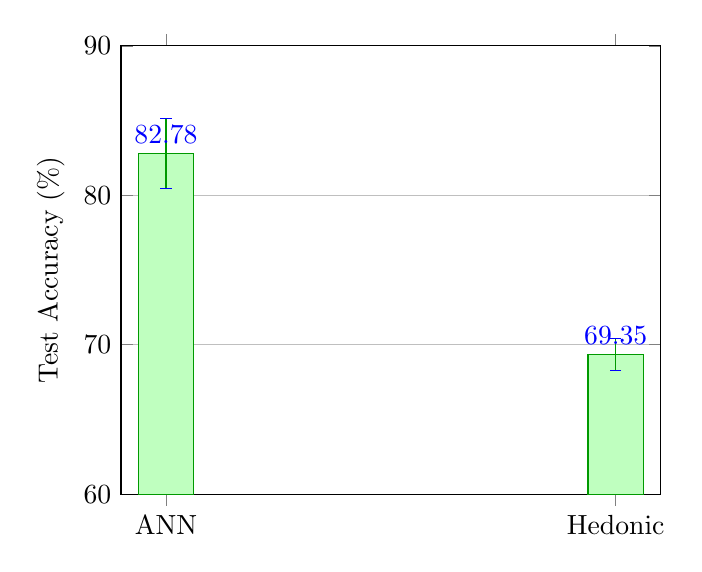
\begin{tikzpicture}
\begin{axis}[
  ybar,
  bar width=20pt,
  ylabel={Test Accuracy (\%)},
  symbolic x coords={ANN,Hedonic},
  xtick=data,
  ymin=60, ymax=90,
  ymajorgrids=true,
  error bars/y dir=both,
  error bars/y explicit,
  nodes near coords,
  nodes near coords align={vertical},
]
\addplot+[fill=green!25, draw=green!60!black] coordinates {
  (ANN,\AnnTimeAccMean) +- (0,\AnnTimeAccStd)
  (Hedonic,\HedTimeAccMean) +- (0,\HedTimeAccStd)
};
\end{axis}
\end{tikzpicture}
\caption{Time split accuracy.}
\end{subfigure}
\caption{Baseline (hedonic) vs primary neural model (ANN) across random and time-based splits (mean $\pm$ std across seeds/splits).}
\label{fig:baseline-vs-ann}
\end{figure}

\subsection{Robustness across seeds and split seeds}
We rerun the same hedonic baseline configuration across multiple model seeds and multiple split seeds to confirm results are not due to a favorable partition.

\begin{figure}[h]
\centering
\begin{subfigure}{0.49\linewidth}
\centering
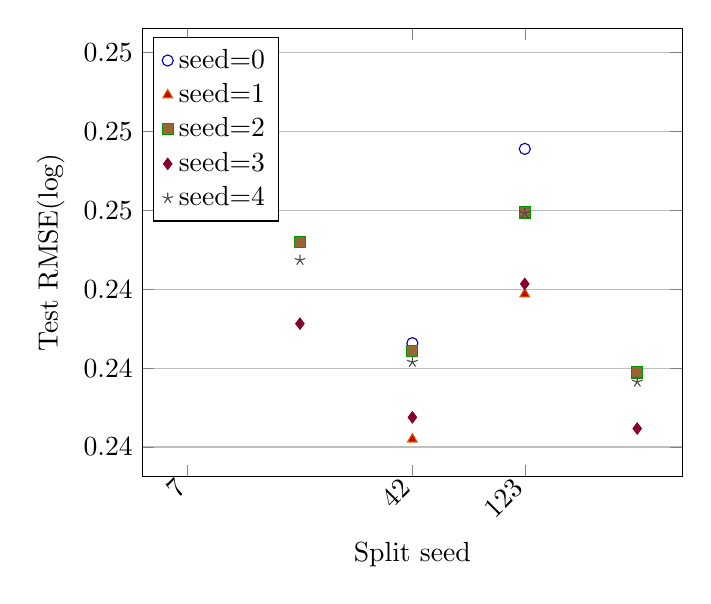
\begin{tikzpicture}
\begin{axis}[
  xlabel={Split seed},
  ylabel={Test RMSE(log)},
  symbolic x coords={7,13,42,123,2024},
  xtick=data,
  x tick label style={rotate=45,anchor=east},
  ymajorgrids=true,
  legend style={at={(0.02,0.98)},anchor=north west},
]
\addplot+[only marks, mark=o, color=blue!70!black] coordinates {
  (7,0.249675) (42,0.242633) (123,0.247562)
};
\addlegendentry{seed=0}
\addplot+[only marks, mark=triangle*, color=orange!80!black] coordinates {
  (7,0.248027) (42,0.240197) (123,0.243877)
};
\addlegendentry{seed=1}
\addplot+[only marks, mark=square*, color=green!60!black] coordinates {
  (7,0.249352) (13,0.245189) (42,0.242437) (123,0.245949) (2024,0.241890)
};
\addlegendentry{seed=2}
\addplot+[only marks, mark=diamond*, color=purple!70!black] coordinates {
  (7,0.247490) (13,0.243128) (42,0.240751) (123,0.244137) (2024,0.240467)
};
\addlegendentry{seed=3}
\addplot+[only marks, mark=star, color=black!70] coordinates {
  (7,0.249071) (13,0.244738) (42,0.242153) (123,0.245933) (2024,0.241649)
};
\addlegendentry{seed=4}
\end{axis}
\end{tikzpicture}
\caption{Random split robustness points (hedonic).}
\end{subfigure}
\hfill
\begin{subfigure}{0.49\linewidth}
\centering
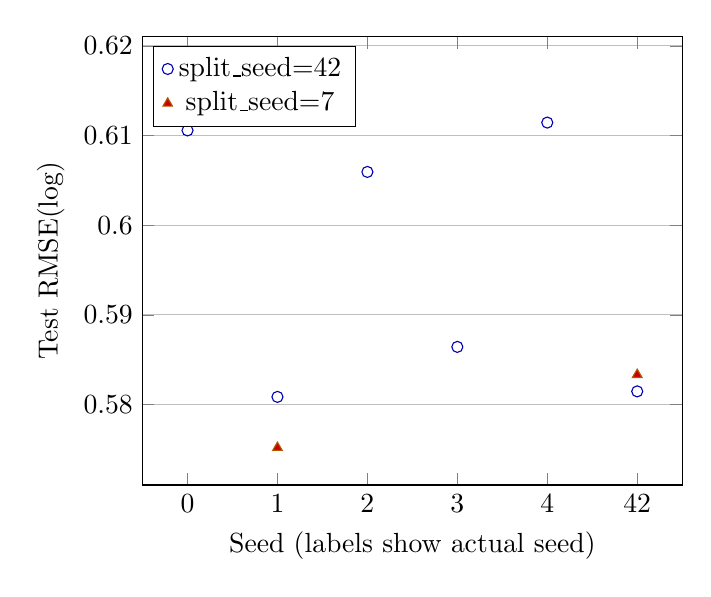
\begin{tikzpicture}
\begin{axis}[
  xlabel={Seed (labels show actual seed)},
  ylabel={Test RMSE(log)},
  xmin=-0.5, xmax=5.5,
  xtick={0,1,2,3,4,5},
  xticklabels={0,1,2,3,4,42},
  ymajorgrids=true,
  legend style={at={(0.02,0.98)},anchor=north west},
]
\addplot+[only marks, mark=o, color=blue!70!black] coordinates {
  (0,0.610566) (1,0.580844) (2,0.605935) (3,0.586421) (4,0.611438) (5,0.581459)
};
\addlegendentry{split\_seed=42}
\addplot+[only marks, mark=triangle*, color=orange!70!black] coordinates {
  (0,0.616849) (1,0.575182) (5,0.583321)
};
\addlegendentry{split\_seed=7}
\end{axis}
\end{tikzpicture}
\caption{Time split sensitivity (hedonic).}
\end{subfigure}
\caption{Robustness plots for the hedonic baseline from \texttt{eval\_suite} runs (logged in \texttt{results\_all.csv}).}
\label{fig:hedonic-robustness}
\end{figure}

\section{Learning curves (quantitative, per-epoch)}
\begin{figure}[h]
\centering
\begin{subfigure}{0.49\linewidth}
\centering
\begin{tikzpicture}
\begin{axis}[
  xlabel={Epoch},
  ylabel={RMSE(log)},
  xmin=1, xmax=20,
  ymajorgrids=true,
  legend style={at={(0.02,0.98)},anchor=north west},
]
\addplot+[mark=*, mark size=1.2pt, color=blue!70!black] table[x=epoch,y=trainrmse] {\HedCurve};
\addlegendentry{Train}
\addplot+[mark=triangle*, mark size=1.2pt, color=orange!80!black] table[x=epoch,y=valrmse] {\HedCurve};
\addlegendentry{Validation}
\end{axis}
\end{tikzpicture}
\caption{RMSE(log) learning curve.}
\end{subfigure}
\hfill
\begin{subfigure}{0.49\linewidth}
\centering
\begin{tikzpicture}
\begin{axis}[
  xlabel={Epoch},
  ylabel={Validation Accuracy (\%)},
  xmin=1, xmax=20,
  ymin=0, ymax=90,
  ymajorgrids=true,
]
\addplot+[mark=*, mark size=1.2pt, color=green!60!black] table[x=epoch,y=valacc] {\HedCurve};
\end{axis}
\end{tikzpicture}
\caption{Validation accuracy curve (MdAPE-derived).}
\end{subfigure}
\caption{Hedonic baseline learning curves for a representative full-feature run (seed=42).}
\label{fig:hedonic-curves}
\end{figure}

\section{Qualitative results (selected samples and error structure)}
\subsection{Prediction scatter (test set sample)}
\begin{figure}[h]
\centering
\begin{tikzpicture}
\begin{axis}[
  xlabel={True log1p(price)},
  ylabel={Predicted log1p(price)},
  xmin=11.0, xmax=16.0,
  ymin=11.0, ymax=16.0,
  grid=both,
  legend style={at={(0.02,0.98)},anchor=north west},
]
\addplot+[only marks, mark=o, mark size=1.4pt, color=blue!60!black] table[x=true,y=pred] {\HedScatter};
\addlegendentry{Hedonic (sample)}
\addplot+[domain=11:16, samples=2, color=black!60] {x};
\addlegendentry{Ideal y=x}
\end{axis}
\end{tikzpicture}
\caption{Predicted vs true values in log space (150 sampled test points).}
\label{fig:hedonic-scatter}
\end{figure}

\subsection{Residual distribution}
\begin{figure}[h]
\centering
\begin{tikzpicture}
\begin{axis}[
  ybar,
  bar width=6pt,
  xlabel={Residual (pred\_log − true\_log)},
  ylabel={Count},
  xmin=-1.05, xmax=1.05,
  ymajorgrids=true,
]
\addplot+[fill=blue!20, draw=blue!60!black] table[x=center,y=count] {\HedResidHist};
\end{axis}
\end{tikzpicture}
\caption{Residual histogram on the test set (log1p space).}
\label{fig:hedonic-residuals}
\end{figure}

\subsection{Error by time (TransactionYear)}
\begin{figure}[h]
\centering
\begin{tikzpicture}
\begin{axis}[
  ybar,
  bar width=14pt,
  xlabel={TransactionYear (test subset)},
  ylabel={Accuracy (\%)},
  symbolic x coords={2010,2011,2012,2013,2014,2015,2016,2017,2018,2019},
  xtick=data,
  x tick label style={rotate=45,anchor=east},
  ymin=84, ymax=91,
  ymajorgrids=true,
]
\addplot+[fill=green!20, draw=green!60!black] table[x=year,y=acc] {\HedByYear};
\end{axis}
\end{tikzpicture}
\caption{Hedonic accuracy by transaction year (random-split test set; years 2010--2019 with \(\ge\)2000 samples).}
\label{fig:hedonic-by-year}
\end{figure}

\subsection{Error by property size (LivingArea deciles)}
\begin{figure}[h]
\centering
\begin{tikzpicture}
\begin{axis}[
  xlabel={LivingArea decile (1=smallest, 10=largest)},
  ylabel={Accuracy (\%)},
  xmin=1, xmax=10,
  ymin=84, ymax=91,
  grid=both,
  xtick={1,2,3,4,5,6,7,8,9,10},
]
\addplot+[mark=*, color=purple!60!black] table[x=decile,y=acc] {\HedByAreaDecile};
\end{axis}
\end{tikzpicture}
\caption{Hedonic accuracy by LivingArea decile (random-split test set).}
\label{fig:hedonic-by-area}
\end{figure}

\subsection{Interpretability: numeric coefficients and location effects}
\paragraph{Numeric coefficients (standardized features).}
Because numeric inputs are standardized, coefficients represent the effect on \(\texttt{log1p(price)}\) per one-standard-deviation increase in that feature.

\begin{figure}[h]
\centering
\begin{subfigure}{0.49\linewidth}
\centering
\begin{tikzpicture}
\begin{axis}[
  xbar,
  xlabel={Coefficient (Δlog1p(price) per 1 std)},
  ytick=data,
  yticklabels={
    LivingArea,
    TransactionYear,
    gcode\_Lon,
    Bath\_Full,
    LandValue,
    Parking\_Count,
    ReplacementCost,
    Bed\_Full,
    gcode\_Lat,
    EntranceCount,
    LotSize,
    Bath\_Half
  },
  ymin=-0.5, ymax=11.5,
  height=8cm,
  grid=both,
]
\addplot+[fill=blue!20, draw=blue!60!black] coordinates {
  (0.226069,0)
  (0.183232,1)
  (0.099802,2)
  (0.046871,3)
  (-0.034840,4)
  (0.031434,5)
  (-0.030806,6)
  (0.028922,7)
  (-0.024763,8)
  (0.020604,9)
  (0.018532,10)
  (0.015635,11)
};
\end{axis}
\end{tikzpicture}
\caption{Top numeric coefficients by magnitude.}
\end{subfigure}
\hfill
\begin{subfigure}{0.49\linewidth}
\centering
\begin{tikzpicture}
\begin{axis}[
  ybar,
  bar width=12pt,
  ylabel={Centered fixed effect (Δlog1p(price))},
  symbolic x coords={M5R,M4N,M4V,M5P,M4W,M4T,M5N,M5M,K0K,L1B,L9Y,L4N,K9A,N0H,L0K,L0M},
  xtick=data,
  x tick label style={rotate=60,anchor=east},
  ymajorgrids=true,
]
\addplot+[fill=orange!25, draw=orange!70!black] table[x=fsa,y=eff] {\HedFsaEffects};
\end{axis}
\end{tikzpicture}
\caption{Centered FSA fixed effects (examples).}
\end{subfigure}
\caption{Interpretability views for the hedonic baseline. Fixed effects are centered within the \texttt{FSA} column for readability.}
\label{fig:hedonic-interpret}
\end{figure}

\subsection{Selected cleaned test samples (good/typical/hard)}
Table~\ref{tab:hedonic-examples} shows three representative test examples selected by absolute percentage error percentile (p5/p50/p95). Values are from the same tensorized dataset used for training.

\begin{table}[h]
\centering
\small
\begin{tabularx}{\linewidth}{@{}lrrrrrll@{}}
\toprule
Example & True price & Pred price & APE (\%) & Year & LivingArea & FSA & City \\
\midrule
Good (p5) & 459{,}500 & 464{,}720 & 1.136 & 2011 & 2{,}388 & L4P & KESWICK \\
Typical (p50) & 800{,}000 & 701{,}701 & 12.287 & 2016 & 2{,}700 & L1T & AJAX \\
Hard (p95) & 1{,}325{,}000 & 1{,}928{,}990 & 45.584 & 2018 & 3{,}286 & L6L & OAKVILLE \\
\bottomrule
\end{tabularx}
\caption{Selected test samples (hedonic baseline). APE is absolute percentage error in price space.}
\label{tab:hedonic-examples}
\end{table}

\section{Challenges and limitations (baseline-specific)}
\begin{itemize}[leftmargin=*]
  \item \textbf{High-cardinality categoricals:} fixed effects for columns like \texttt{PropertyStyle} and \texttt{gcode\_City} require large embedding tables; rare categories can be noisy.
  \item \textbf{Identifiability of fixed effects:} fixed-effect tables are not uniquely identified (bias and per-category offsets can shift). For interpretability, we center effects within a column before plotting (Figure~\ref{fig:hedonic-interpret}).
  \item \textbf{Time-based generalization:} under time splits, hedonic regression degrades substantially (Figure~\ref{fig:baseline-vs-ann}), indicating limited ability to extrapolate changing market conditions.
  \item \textbf{Preprocessing leakage:} current tensorization computes numeric mean/std and categorical vocab on the full dataset; a stricter pipeline would compute these on train only per split.
\end{itemize}

\section{Plan for testing on never-before-seen data}
\begin{itemize}[leftmargin=*]
  \item \textbf{Preferred: fresh RPS extract.} Hold out a new, later time window (e.g., post-2025 transactions) not used during model development, and evaluate the frozen baseline and ANN once on this dataset.
  \item \textbf{Fallback: external dataset.} If new internal transactions cannot be obtained, evaluate on an entirely different public housing-sales dataset (different region/source) to test robustness of learned relationships.
\end{itemize}

\section*{Repro commands}
\begin{lstlisting}[language=bash]
# 1) Build full-feature tensors (from the cleaned CSV)
python prepare_ann_tensors.py --csv cleaned_transaction_gtha-2.csv \
  --out ann_tensors_full.pt --feature-set full

# 2) Train/evaluate hedonic baseline (random split)
python hedonic_baseline.py --data ann_tensors_full.pt --split-strategy random \
  --epochs 20 --batch-size 8192 --lr 0.01 --weight-decay 0.0 --seed 42 \
  --out-csv hedonic_results.csv

# 3) Merge into the single canonical results sheet
python export_results.py
\end{lstlisting}

\end{document}
